\section{\Simple{} Attacks}\label{sec:attack_setup}

In this section, we discuss \simple{} attacks, i.e., exploits in which the trifecta appears within a single page.
We find several such potential \simple{} exploits in the Linux kernel. We detail such an example in the FireWire driver, as this is the hardware we have in our setup. 



\subsection{Attack setup}
In our attacks, we use a 28 core, Dell PowerEdge R730 server, an Intel x86 machine with Ubuntu 18.04 (kernel version 4.15), as our victim machine. The server is equipped with Intel VT-d IOMMU, a Broadcom NetXtreme II BCM5709 Gigabit Ethernet NIC, a Mellanox Technologies ConnectX-4 Ethernet NIC and VIA Technologies, Inc. VT6315 Series Firewire Controller. An identical machine connected to the victim with a FireWire cable acting as the attacker. 

We create a malicious FireWire device by modifying the Linux-IO Target (LIO) subsystem on the attacker machine. The LIO subsystem supports hard disk emulation for remote computers via the \spb{} protocol; and, as such, is a suitable platform to execute such attacks. 

We implement multiple attacks against the Linux kernel network stack. In order to demonstrate an attack by a malicious NIC, we use a FireWire device similarly to \cite{SLND10}. To emulate an attack by a malicious NIC using a FireWire device, we create an \iova{} page table sharing between the FireWire and the actual NIC. A minor patch is needed for the victim OS to facilitate this emulation. This way, the attacker machine can access the same pages as the NIC. This allows us to execute an attack using a programmable interface, emulating a malicious NIC.

\subsection{FireWire Background}

The FireWire protocol is a serial replacement for the parallel SCSI bus, which provides connectivity for digital audio and video equipment. The SBP-2 (serial bus protocol $\#2$) enables the use of SCSI devices over Firewire. 

While Firewire is a somewhat outdated physical connector, rarely in use for modern systems, some cables allow seamless conversion between Firewire and Thunderbolt. This allows for Firewire use in modern setups.

A SCSI connection consists of two endpoints: an initiator' (i.e., OS), which initiates SCSI session, and a target (i.e., a disk), which holds for the initiator's commands and provides the required I/O data transfers. 

Linux has a Linux-IO (LIO) module, which allows for a Linux machine to act as a SCSI target. One can boot the machine in \emph{target disk mode}, such that it acts as a disk (i.e., SCSI target) when connected to another computer. When the connection is via FireWire, the SPB2 protocol is used.

\subsection{Linux FireWire Exploit} \label{sec:sbp2_attack}
\begin{figure}
    \centering
    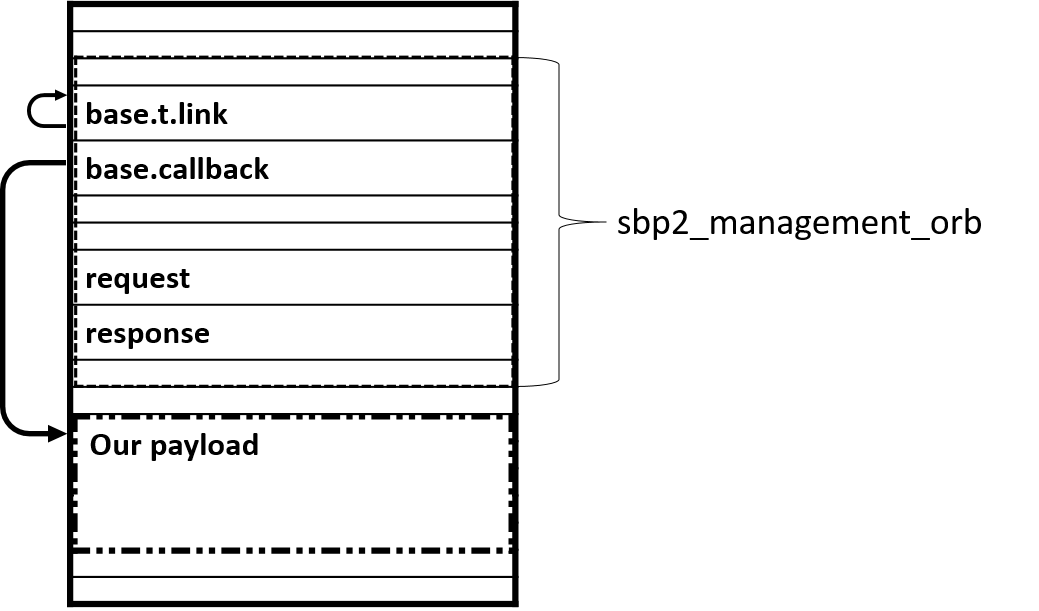
\includegraphics[width=1\linewidth]{figs/sbp.png}
    \caption{\texttt{spb2\_management\_orb} struct with fields relevant to the DMA attack.}
    \label{fig:orb}
\end{figure}

The Linux FireWire driver has a type (a) (Fig. \ref{fig:colocation} (a)) \subpage{} vulnerability and the exploit we demonstrate, falls under the category of a \simple{} attack. Both the device metadata and the I/O buffers for the \spb{} protocol implemented by the spb2 driver are contained inside the \texttt{spb2\_management\_orb} struct (Fig. \ref{fig:orb}). This provides the attacker with both \means{} and \oportunity{}.

To enable communication between the initiator and the target, the spb2 driver maps the request and response fields. As a result, the whole 4~KB page, that contains the \texttt{spb2\_management\_orb} struct is accessible with both READ and WRITE to the device. Read access is available via the \iova{} created when the \emph{request} was mapped. Write access is available via the \iova{} created when the \emph{response} was mapped. Consequently, the device can read and manipulate both the request and response fields as well as the metadata. 

Additionally, the \texttt{spb2\_management\_orb} struct contains a callback function \texttt{base.callback} which provides the \oportunity{}. Generally, to preserve normal device behavior, the original callback should also be called before or after the malicious code. However, in our experiments, we have found that ignoring the original callback has no ill side effects. 

The \texttt{spb2\_management\_orb} struct also holds its own address in the \texttt{base.t.link} field, and thus provides the attacker with \means{}. At this point, the attacker can create a \mabaf{} on the same page and complete the MMO trifecta. 

The code of the \mabaf{} appears in Appendix \ref{apx:shellcode}. It is also important to note that in this attack KASLR was irrelevant, as the critical \kva{} appeared in full, inside the readable page.

\smallskip
\noindent \textbf{Remark 1.} To date (kernel 5.3), the \texttt{spb2\_management\_orb} struct has not changed.

\smallskip
\noindent\textbf{Remark 2.} An additional such exploit also appear in nvme\_fc driver via the \texttt{struct nvmefc\_ls\_req}. The difference in detailing such an exploit would extend only to the struct field names.